%
%	 untitled
%
%	 Created by Jesper Josefsson on 2011-10-10.
%	 Copyright (c) 2011 __MyCompanyName__. All rights reserved.
%
\documentclass[]{article}

% Use utf-8 encoding for foreign characters
\usepackage[utf8]{inputenc}

% Setup for fullpage use
\usepackage{fullpage}

% Uncomment some of the following if you use the features
%
% Running Headers and footers
\usepackage{fancyhdr}

% Multipart figures
%\usepackage{subfigure}

% More symbols
\usepackage{amsmath}
\usepackage{amssymb}
\usepackage{latexsym}

% Surround parts of graphics with box
\usepackage{boxedminipage}

% Package for including code in the document
\usepackage{listings}

% If you want to generate a toc for each chapter (use with book)
\usepackage{minitoc}

% This is now the recommended way for checking for PDFLaTeX:
\usepackage{ifpdf}

%\newif\ifpdf
%\ifx\pdfoutput\undefined
%\pdffalse % we are not running PDFLaTeX
%\else
%\pdfoutput=1 % we are running PDFLaTeX
%\pdftrue
%\fi

\ifpdf
\usepackage[pdftex]{graphicx}
\else
\usepackage{graphicx}
\fi
\title{SSY080 \\ Inlämningsuppgift}
\author{
Linus Oleander - 880613 - 4873 \\
Jesper Josefsson - 860409 - 5276 
}

\date{2011-10-10}

\begin{document}

\ifpdf
\DeclareGraphicsExtensions{.pdf, .jpg, .tif}
\else
\DeclareGraphicsExtensions{.eps, .jpg}
\fi

\maketitle

\section{Bakgrund}
Uppgiften går ut på att genomföra ett antal experiment gällande generering och behandling av signaler med Matlab.

\section{Generering av fyrkantsvåg med hjälp av Fourierserie - (3.1)}
\subsection{Fourierkoefficienter} % (fold)
\label{sub:fourierkoefficienter}
Den första uppgiften var att ta fram ett slutet uttryck för Fourierseriekoefficienterna $A_k$ och $B_k$.\\
Vi använde följande samband:\\
\begin{align*}
	C_k &= \frac{1}{T} \int_0^T \! x(t) e^{-jk\omega_0 t}\, \mathrm{d} t =\\
			&= \frac{1}{T} \left(
						\int_0^{\frac{T}{2}} \! e^{-jk\omega_0 t}\, \mathrm{d} t
						- \int_{\frac{T}{2}}^T \! e^{-jk\omega_0 t}\, \mathrm{d} t \right) =\\
			&= \frac{1}{-jk\omega_0 T} \left(
						\left[e^{-jk\omega_0 t}\right]_0^{\frac{T}{2}}
						- \left[e^{-jk\omega_0 t}\right]_{\frac{T}{2}}^T
					\right) = \\
			&= \left[
					\omega = \frac{2\pi}{T} \Rightarrow \frac{\omega_0 T}{2} = \pi ,\;	\omega_0 T = 2\pi
				\right] = \\
			&= \frac{1}{-jk\omega_0 T} \left(
					2e^{-jk\pi} - e^{-jk2\pi} - 1
				\right) = \\
			&=	\left[
					\begin{array}{ll}
						2e^{-jk\pi} &=
							\left\{
								\begin{array}{ll}
									-2	& ,k\text{ udda} \\
									2 & ,k\text{ jämn} 
								\end{array}
							\right. \\
						e^{-jk2\pi} &= 1
					\end{array}
					\right] = \\ \\
			&= \left\{ \begin{array}{ll}
						\frac{-4}{-jk2\pi} = \frac{2}{jk\pi} = -\frac{2j}{k\pi}&,k\text{ udda} \\
						0 &,k\text{ jämn}
					\end{array} \right.\\
	A_k &= C_k - C_{-k} = -\frac{2i}{k\pi} + \frac{2i}{k\pi} = 0\\
	C_k &= \frac{1}{2}(A_k - iB_k) \Rightarrow B_k = 2iC_k = \frac{4}{k\pi}\\
\end{align*}
% subsection fourierkoefficienter (end)

\subsection{Generering av fyrkantsvåg} % (fold)
Vi använder Fourierkoefficienterna för att generera en fyrkantsvåg i matlab med hjälp av definitionen av Fourierserien på trigonometrisk form: 
\[
	x(t) = A_0 + \sum\limits_{k=1}^\infty [A_k cos(k\omega_0 t) + B_k sin(k\omega_0 t)] \\
\]

Koden blir som nedan:

\begin{verbatim}
T = 2;
w=2*pi/T;
M=200;
t=T*(0:M-1)/M;
y = @(t) 0;
bs = [];
for k=1:100
		ck = -(mod(k, 2))*((1i*2)/(pi*k));
		cminusk = -(mod(k, 2))*((1i*2)/(pi*(-k)));
		ak = ck + cminusk;
		bk = 2i*ck;
		bs = [bs bk];
		y = @(t) y(t) + ak*cos(k*w*t) + bk*sin(k*w*t);
end
\end{verbatim}
\begin{figure}[htb]
  \centering
  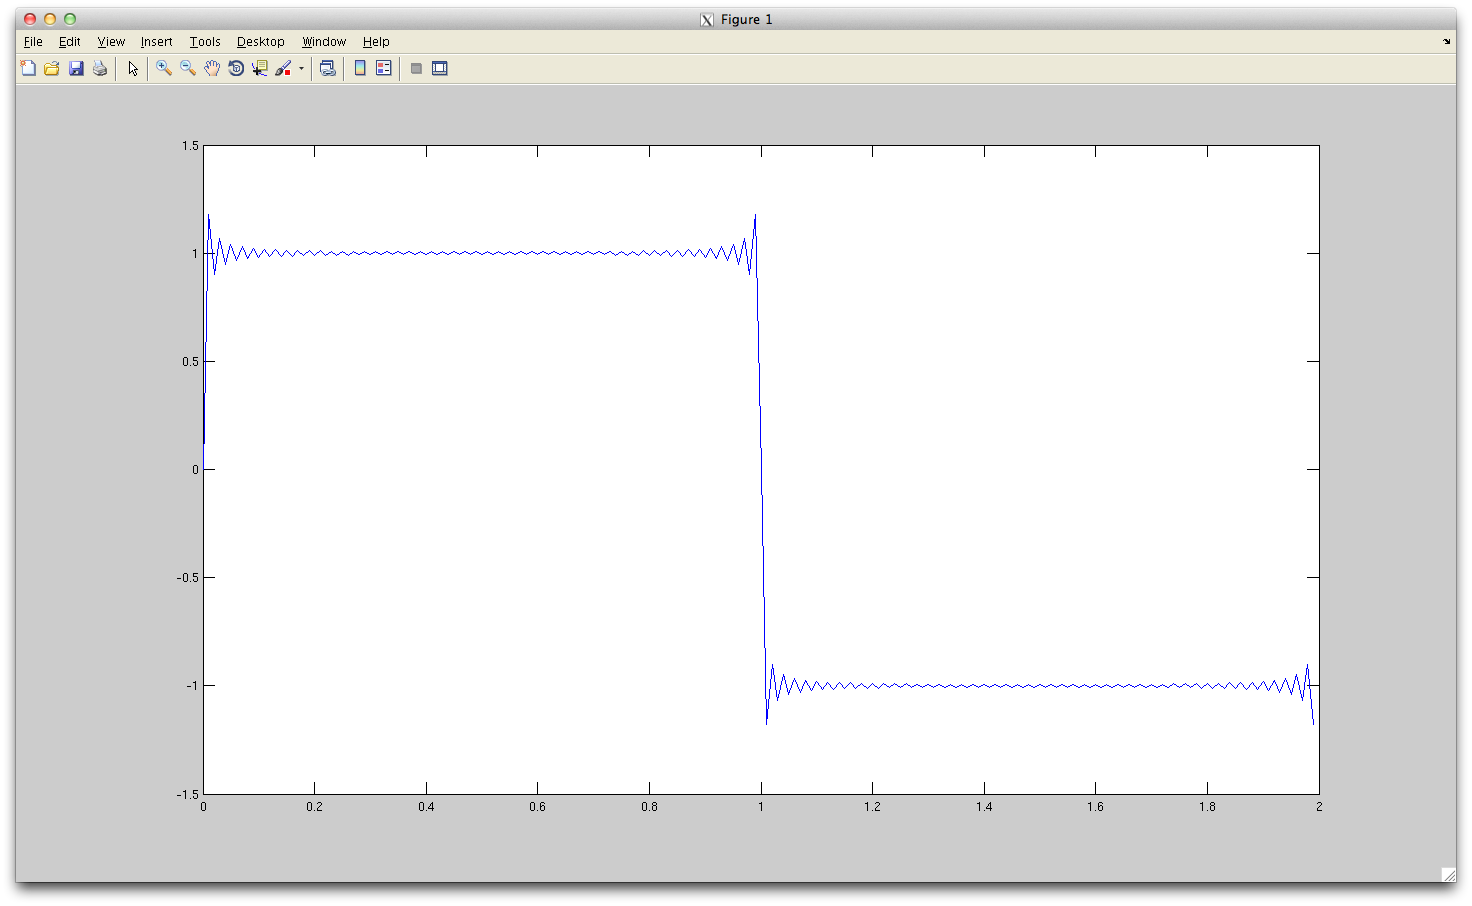
\includegraphics[width=15.0cm]{square.png}
  \caption{Vår fyrkantsvåg}
\end{figure}
% subsection generering_av_fyrkantsvåg (end)

\subsection{Linjära system och sinusar (3.2)} % (fold)
\label{sub:linjära_system_och_sinusar_3_2_}

% subsection linjära_system_och_sinusar_3_2_ (end)
\bibliographystyle{plain}
\bibliography{}
\end{document}
